\subsection{Sentences and punctuation statistics}

We then did some statistics on the sentences and the punctuation. We started by analysing the average length of the sentences (see figure  \ref{average_sent_length_figure}).

\begin{figure}[H]
	\centering
    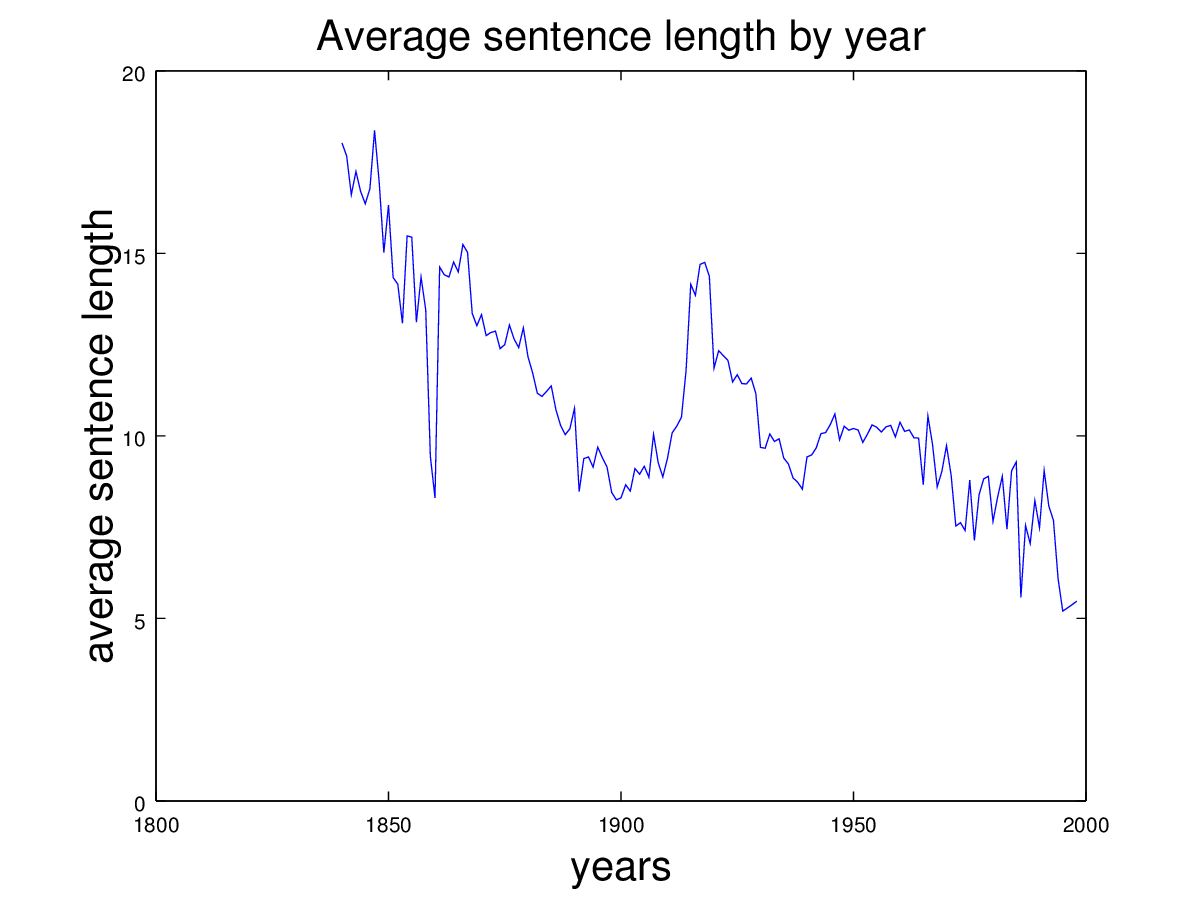
\includegraphics[scale=0.5]{Pictures/statistics/sentences-length/means.png}
    \caption{Average length of sentences by year}
    \label{average_sent_length_figure}\hfill
\end{figure}

\begin{figure}[H]
	\centering
    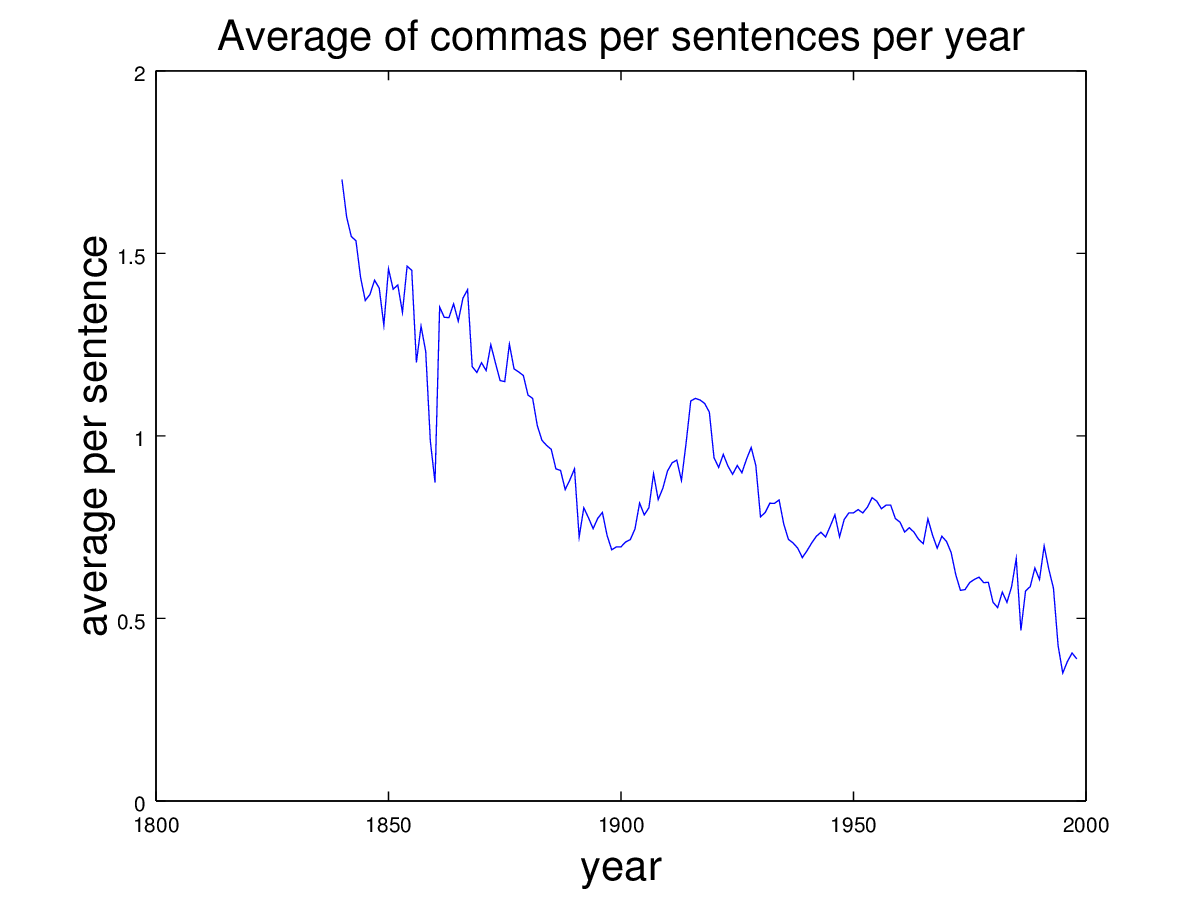
\includegraphics[scale=0.5]{Pictures/statistics/punctuation/graph.png}
    \caption{Average number of commas, semicolons and colons per sentence per year}
    \label{average_punct}\hfill
\end{figure}

If we forget the down peak near 1850, which comes from some unknown problem in two year (maybe less articles, maybe big OCR problems) we see that the length of the sentences tends to decrease. Actually, it decreases quite a lot, going from 15-20 words sentences in 1840 down to 8-10 words sentences in 1990.

(Note : another problem than the bad OCR is that from year 1917 to 1919 (included), only one of the two newspapers has articles, so this affects the statistics for those years as there are less articles than in the other years).

We can correlate those results with the statistics on punctuation. In figure \ref{average_punct}, the black curve represents the average of commas per sentences per year, the red curve the average of semicolons and the blue curve the average of colons. The two last curves are not really interesting as they do not vary much, we use approximatly the same number of colons and semicolons in 1990 as in 1840. The black curve however is interesting, we tend to use less commas, this is quite logical, as we make shorter sentences, we need to use less commas.\\

Again those statistics show the lignuistic drift, between 1840 and 1990 we make shorter sentences, which affects the punctuation we use. \\

As those observations shows a real variation between year we thought it could be a good idea to use them for a metric, the result is presented in a next section.